\SourceLeaf{179}Ein grosser Theil der Schrift dreht sich um die Behauptung gegen \textsc{Kant}, dass die
Gewissheit der Geometrie sich nicht auf Anschauung, sondern auf Definitionen und auf das
»Principium identitatis« und das »Principium contradictionis« gründe. Dass von diesen
logischen Hülfsmitteln zur Einkleidung und Verkettung der Wahrheiten in der Geometrie fort
und fort Gebrauch gemacht werde, hat wohl \textsc{Kant} nicht läugnen wollen: aber dass
dieselben für sich nichts zu leisten vermögen, und nur taube Blüthen treiben, wenn nicht die
befruchtende lebendige Anschauung des Gegenstandes selbst überall waltet, kann wohl niemand
verkennen, der mit dem Wesen der Geometrie vertraut ist. Hrn. \textsc{Schwabs} Widerspruch
scheint übrigens zum Theil nur auf Missverständniss zu beruhen: wenigstens scheint uns, nach
dem 16ten Paragraph seiner Schrift, welcher von Anfang bis zu Ende gerade das
Anschauungsvermögen in Anspruch nimmt, und am Ende beweisen soll, »postulata Euclidis in
generaliora resolvi posse, non sensu et \textls{intuitione} sed \textls{intellectu} fundata«, dass Hr.
\textsc{Schwab} sich bei diesen Benennungen verschiedener Zweige des Erkenntnissvermögens
etwas anderes gedacht haben müsse, als der Königsberger Philosoph.

Obgleich der Verfasser der zweiten Schrift seinen Gegenstand auf eine ganz andere und
wirklich mathematische Art behandelt hat, so können wir doch über das Resultat derselben
nicht günstiger urtheilen. Wir haben nicht die Absicht, hier den ganzen Gang seines
versuchten Beweises darzulegen, sondern begnügen uns, dasjenige hier herauszuheben, worauf
im Grunde alles ankommt.

\begin{center}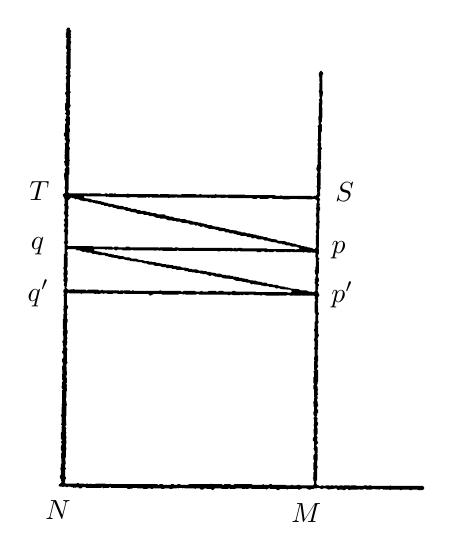
\begin{tikzpicture}[x=0.00759494cm,y=-0.00759494cm]
\fill[even odd rule] (98,28) -- (96,31) -- (96,36) -- (95,37) -- (95,44) -- (97,46) -- (96,48) -- (96,58) -- (95,59) -- (95,62) -- (97,64) -- (97,68) -- (96,69) -- (96,72) -- (97,73) -- (96,75) -- (96,88) -- (97,90) -- (95,93) -- (95,95) -- (96,96) -- (96,103) -- (95,105) -- (97,107) -- (97,108) -- (95,110) -- (95,113) -- (96,114) -- (96,120) -- (95,121) -- (96,134) -- (94,137) -- (94,139) -- (95,140) -- (95,143) -- (96,144) -- (96,146) -- (95,147) -- (95,150) -- (96,152) -- (94,155) -- (94,165) -- (96,169) -- (94,171) -- (94,172) -- (96,174) -- (96,176) -- (95,177) -- (95,180) -- (94,181) -- (94,183) -- (95,184) -- (95,188) -- (94,189) -- (94,202) -- (92,205) -- (92,208) -- (94,211) -- (93,214) -- (95,217) -- (95,220) -- (93,222) -- (94,224) -- (94,231) -- (93,232) -- (94,234) -- (93,236) -- (94,238) -- (93,240) -- (93,247) -- (94,248) -- (94,250) -- (92,252) -- (93,254) -- (93,257) -- (95,260) -- (95,262) -- (93,265) -- (94,269) -- (92,273) -- (93,283) -- (94,284) -- (94,293) -- (93,294) -- (93,297) -- (94,298) -- (94,304) -- (90,307) -- (90,309) -- (92,311) -- (92,313) -- (93,314) -- (93,323) -- (92,324) -- (93,326) -- (93,335) -- (92,336) -- (92,339) -- (93,340) -- (94,346) -- (92,349) -- (92,351) -- (93,352) -- (93,356) -- (92,357) -- (92,359) -- (93,360) -- (93,365) -- (92,366) -- (92,369) -- (93,370) -- (93,385) -- (92,386) -- (92,388) -- (93,389) -- (93,406) -- (92,407) -- (92,428) -- (91,429) -- (91,431) -- (92,432) -- (92,437) -- (91,438) -- (92,448) -- (91,449) -- (91,451) -- (93,454) -- (92,456) -- (92,459) -- (93,460) -- (93,465) -- (91,467) -- (91,470) -- (92,471) -- (92,474) -- (91,475) -- (92,477) -- (92,493) -- (91,494) -- (92,496) -- (91,498) -- (92,506) -- (91,507) -- (91,515) -- (90,516) -- (90,531) -- (91,532) -- (91,534) -- (90,535) -- (90,542) -- (91,543) -- (91,550) -- (89,553) -- (90,555) -- (90,560) -- (91,561) -- (91,563) -- (90,564) -- (90,568) -- (89,569) -- (89,571) -- (91,574) -- (91,579) -- (89,582) -- (89,587) -- (90,588) -- (90,593) -- (89,594) -- (89,600) -- (90,601) -- (89,603) -- (90,605) -- (89,607) -- (89,616) -- (90,617) -- (90,619) -- (89,620) -- (89,626) -- (88,627) -- (88,630) -- (90,632) -- (90,633) -- (89,634) -- (89,657) -- (88,658) -- (89,661) -- (88,662) -- (88,674) -- (87,675) -- (87,677) -- (88,678) -- (88,689) -- (87,691) -- (89,693) -- (88,695) -- (88,704) -- (87,705) -- (87,715) -- (89,717) -- (89,718) -- (87,720) -- (88,722) -- (88,726) -- (87,727) -- (87,734) -- (88,735) -- (88,739) -- (87,740) -- (88,756) -- (87,757) -- (87,763) -- (86,764) -- (86,766) -- (87,767) -- (87,775) -- (85,777) -- (85,780) -- (87,783) -- (88,788) -- (85,791) -- (84,791) -- (83,793) -- (85,795) -- (89,795) -- (90,796) -- (92,795) -- (95,795) -- (96,796) -- (98,796) -- (99,795) -- (103,795) -- (104,796) -- (107,796) -- (108,797) -- (116,796) -- (118,798) -- (121,798) -- (123,796) -- (128,796) -- (129,797) -- (154,797) -- (156,796) -- (158,798) -- (160,797) -- (167,797) -- (168,796) -- (170,796) -- (171,797) -- (197,797) -- (199,799) -- (207,798) -- (208,797) -- (214,797) -- (215,798) -- (224,798) -- (225,799) -- (231,799) -- (232,798) -- (237,798) -- (238,799) -- (240,799) -- (241,798) -- (254,798) -- (255,799) -- (259,799) -- (260,798) -- (268,798) -- (269,799) -- (273,799) -- (274,798) -- (280,798) -- (281,797) -- (283,798) -- (285,797) -- (289,797) -- (290,798) -- (293,797) -- (294,798) -- (310,798) -- (311,799) -- (313,798) -- (319,798) -- (321,800) -- (324,800) -- (327,798) -- (330,798) -- (331,799) -- (338,799) -- (340,801) -- (341,801) -- (344,798) -- (355,798) -- (356,799) -- (366,799) -- (367,798) -- (369,798) -- (370,799) -- (378,799) -- (379,798) -- (389,798) -- (390,799) -- (394,799) -- (396,798) -- (397,799) -- (400,799) -- (401,798) -- (405,798) -- (406,799) -- (429,799) -- (430,800) -- (434,798) -- (436,798) -- (437,799) -- (446,799) -- (447,800) -- (451,801) -- (453,799) -- (464,799) -- (465,800) -- (467,799) -- (483,799) -- (484,800) -- (486,800) -- (490,798) -- (497,798) -- (501,800) -- (504,800) -- (505,799) -- (509,799) -- (510,798) -- (514,798) -- (515,797) -- (518,797) -- (522,799) -- (524,799) -- (525,798) -- (530,798) -- (534,800) -- (547,798) -- (550,801) -- (552,800) -- (558,800) -- (559,801) -- (561,801) -- (564,799) -- (566,799) -- (568,801) -- (570,801) -- (571,800) -- (584,800) -- (585,799) -- (587,800) -- (592,800) -- (593,799) -- (596,799) -- (597,800) -- (606,800) -- (607,799) -- (620,800) -- (621,799) -- (624,799) -- (625,800) -- (636,800) -- (637,801) -- (639,800) -- (653,800) -- (654,801) -- (656,801) -- (657,800) -- (669,800) -- (670,801) -- (673,801) -- (674,800) -- (683,800) -- (684,801) -- (691,801) -- (694,799) -- (694,796) -- (692,794) -- (639,794) -- (638,793) -- (636,794) -- (606,794) -- (605,793) -- (602,793) -- (601,794) -- (599,794) -- (598,793) -- (594,793) -- (593,794) -- (581,794) -- (580,793) -- (572,793) -- (571,794) -- (569,793) -- (560,793) -- (559,794) -- (557,793) -- (553,793) -- (552,794) -- (550,794) -- (549,793) -- (545,793) -- (544,794) -- (542,793) -- (538,793) -- (537,794) -- (535,793) -- (530,793) -- (529,794) -- (526,794) -- (525,793) -- (523,793) -- (522,794) -- (519,794) -- (518,793) -- (516,793) -- (514,791) -- (514,785) -- (515,784) -- (515,765) -- (516,764) -- (516,761) -- (515,760) -- (515,752) -- (516,751) -- (516,741) -- (515,740) -- (516,738) -- (516,730) -- (514,727) -- (514,725) -- (517,722) -- (515,718) -- (515,715) -- (516,713) -- (514,710) -- (516,706) -- (516,698) -- (515,697) -- (515,694) -- (516,693) -- (517,689) -- (515,686) -- (516,681) -- (514,679) -- (514,678) -- (515,677) -- (515,673) -- (517,671) -- (517,668) -- (515,665) -- (515,662) -- (517,660) -- (517,657) -- (516,656) -- (516,653) -- (515,652) -- (515,649) -- (516,648) -- (516,645) -- (515,643) -- (517,641) -- (516,639) -- (516,634) -- (517,633) -- (516,632) -- (516,628) -- (515,627) -- (515,624) -- (516,623) -- (516,620) -- (517,619) -- (517,601) -- (515,599) -- (515,597) -- (517,595) -- (517,593) -- (516,592) -- (516,586) -- (517,585) -- (517,577) -- (516,576) -- (516,566) -- (517,565) -- (517,563) -- (516,562) -- (517,557) -- (516,555) -- (517,554) -- (517,551) -- (516,550) -- (516,547) -- (518,543) -- (518,541) -- (517,540) -- (517,534) -- (516,533) -- (517,531) -- (517,527) -- (516,526) -- (516,524) -- (518,520) -- (517,518) -- (517,508) -- (518,507) -- (518,505) -- (516,503) -- (517,501) -- (516,489) -- (517,488) -- (517,478) -- (519,475) -- (516,468) -- (516,466) -- (517,465) -- (517,460) -- (518,459) -- (518,457) -- (517,456) -- (517,453) -- (518,452) -- (518,447) -- (517,446) -- (517,439) -- (518,438) -- (518,419) -- (517,417) -- (519,415) -- (519,414) -- (517,412) -- (517,407) -- (518,406) -- (518,398) -- (517,396) -- (518,395) -- (518,365) -- (519,364) -- (519,354) -- (520,353) -- (519,351) -- (519,342) -- (518,341) -- (519,339) -- (519,334) -- (520,333) -- (520,328) -- (519,327) -- (519,325) -- (520,324) -- (519,322) -- (519,317) -- (520,316) -- (520,314) -- (518,312) -- (518,311) -- (520,309) -- (520,304) -- (519,302) -- (520,301) -- (520,298) -- (521,297) -- (521,294) -- (520,293) -- (521,291) -- (521,271) -- (520,269) -- (521,268) -- (521,264) -- (522,263) -- (521,249) -- (522,248) -- (522,232) -- (523,231) -- (523,229) -- (522,228) -- (522,221) -- (521,220) -- (521,218) -- (522,217) -- (522,209) -- (521,207) -- (522,206) -- (522,202) -- (523,201) -- (523,190) -- (522,189) -- (522,186) -- (523,185) -- (523,179) -- (524,178) -- (524,162) -- (523,161) -- (523,157) -- (524,156) -- (524,149) -- (523,148) -- (523,144) -- (524,143) -- (525,135) -- (524,134) -- (524,115) -- (523,113) -- (524,112) -- (524,107) -- (525,106) -- (525,103) -- (522,100) -- (521,100) -- (518,104) -- (518,109) -- (519,110) -- (519,118) -- (520,119) -- (519,121) -- (519,132) -- (518,133) -- (518,136) -- (519,137) -- (519,143) -- (520,145) -- (518,149) -- (519,151) -- (519,153) -- (518,154) -- (518,176) -- (517,177) -- (518,190) -- (516,193) -- (517,195) -- (517,214) -- (516,215) -- (516,217) -- (517,218) -- (517,220) -- (516,221) -- (516,226) -- (517,227) -- (517,229) -- (516,230) -- (516,236) -- (517,238) -- (516,239) -- (516,257) -- (515,258) -- (515,261) -- (514,262) -- (514,265) -- (516,269) -- (516,271) -- (515,272) -- (515,276) -- (514,277) -- (515,279) -- (515,292) -- (514,294) -- (515,295) -- (515,302) -- (516,304) -- (515,305) -- (515,307) -- (513,309) -- (510,309) -- (509,310) -- (506,310) -- (505,309) -- (456,309) -- (455,308) -- (453,309) -- (446,309) -- (445,308) -- (395,308) -- (394,307) -- (366,307) -- (364,308) -- (363,307) -- (347,307) -- (346,306) -- (344,307) -- (322,307) -- (321,306) -- (319,306) -- (318,307) -- (313,307) -- (312,306) -- (289,306) -- (288,307) -- (253,306) -- (252,307) -- (250,307) -- (249,306) -- (200,306) -- (199,305) -- (197,306) -- (179,306) -- (178,305) -- (176,305) -- (175,306) -- (173,305) -- (168,305) -- (167,306) -- (165,306) -- (164,305) -- (161,305) -- (160,306) -- (154,306) -- (153,305) -- (134,305) -- (133,306) -- (131,305) -- (101,305) -- (99,303) -- (99,300) -- (100,299) -- (100,274) -- (101,273) -- (101,262) -- (100,261) -- (100,259) -- (101,258) -- (101,251) -- (102,250) -- (101,248) -- (101,232) -- (102,231) -- (102,229) -- (101,228) -- (100,223) -- (101,222) -- (101,219) -- (102,218) -- (102,215) -- (101,214) -- (101,203) -- (102,202) -- (102,197) -- (101,196) -- (101,191) -- (102,190) -- (102,178) -- (101,177) -- (101,174) -- (102,173) -- (102,167) -- (101,166) -- (101,163) -- (103,159) -- (103,157) -- (102,156) -- (102,138) -- (103,137) -- (103,135) -- (102,134) -- (102,111) -- (103,110) -- (103,107) -- (102,106) -- (103,101) -- (102,100) -- (102,98) -- (103,97) -- (103,66) -- (104,65) -- (103,63) -- (103,55) -- (104,54) -- (104,51) -- (103,50) -- (103,46) -- (104,45) -- (103,41) -- (104,39) -- (103,38) -- (103,36) -- (104,35) -- (104,33) -- (102,31) -- (102,29) -- (101,28) -- cycle
(97,473) -- (99,471) -- (100,471) -- (101,472) -- (120,472) -- (121,473) -- (123,472) -- (142,472) -- (143,473) -- (146,473) -- (147,472) -- (149,473) -- (152,473) -- (153,472) -- (157,472) -- (158,473) -- (160,472) -- (164,472) -- (165,473) -- (173,473) -- (174,472) -- (181,472) -- (182,473) -- (190,473) -- (191,472) -- (193,472) -- (194,473) -- (233,473) -- (236,476) -- (242,473) -- (255,473) -- (256,474) -- (283,474) -- (284,473) -- (290,473) -- (291,474) -- (293,473) -- (295,474) -- (313,474) -- (314,473) -- (317,473) -- (318,474) -- (365,474) -- (366,475) -- (369,475) -- (370,474) -- (373,474) -- (374,475) -- (386,475) -- (387,474) -- (389,475) -- (391,475) -- (392,474) -- (400,475) -- (401,474) -- (409,474) -- (410,475) -- (420,475) -- (421,476) -- (425,474) -- (426,475) -- (429,475) -- (430,476) -- (452,476) -- (453,475) -- (455,476) -- (457,476) -- (458,475) -- (460,476) -- (463,476) -- (464,475) -- (469,475) -- (470,476) -- (475,476) -- (476,475) -- (478,476) -- (488,476) -- (489,475) -- (491,476) -- (510,476) -- (512,478) -- (511,480) -- (512,482) -- (512,485) -- (511,486) -- (511,504) -- (512,505) -- (512,508) -- (513,509) -- (512,511) -- (512,519) -- (511,520) -- (511,531) -- (510,532) -- (510,535) -- (511,536) -- (511,547) -- (510,548) -- (510,551) -- (511,552) -- (511,562) -- (510,563) -- (510,565) -- (511,566) -- (511,578) -- (510,579) -- (510,583) -- (511,584) -- (510,586) -- (510,599) -- (511,601) -- (509,603) -- (510,605) -- (510,611) -- (509,612) -- (509,622) -- (510,623) -- (510,625) -- (509,626) -- (509,632) -- (510,633) -- (510,645) -- (511,646) -- (510,648) -- (510,652) -- (509,653) -- (509,657) -- (510,658) -- (509,660) -- (510,662) -- (510,669) -- (509,670) -- (509,674) -- (511,678) -- (509,681) -- (510,683) -- (510,691) -- (509,692) -- (510,694) -- (510,699) -- (509,700) -- (510,711) -- (508,715) -- (508,718) -- (510,720) -- (510,730) -- (509,732) -- (511,736) -- (511,740) -- (509,743) -- (509,750) -- (510,751) -- (510,754) -- (509,755) -- (509,767) -- (510,768) -- (510,770) -- (509,771) -- (509,779) -- (508,781) -- (509,782) -- (509,785) -- (510,786) -- (510,791) -- (508,793) -- (487,793) -- (486,792) -- (482,792) -- (481,793) -- (475,793) -- (474,792) -- (472,792) -- (471,793) -- (463,793) -- (462,792) -- (440,792) -- (439,791) -- (436,791) -- (435,792) -- (426,792) -- (425,791) -- (423,792) -- (407,792) -- (406,791) -- (377,791) -- (376,792) -- (371,792) -- (370,791) -- (360,791) -- (359,792) -- (357,792) -- (356,791) -- (339,791) -- (338,790) -- (336,791) -- (301,791) -- (300,792) -- (287,792) -- (286,791) -- (282,791) -- (281,792) -- (276,792) -- (275,791) -- (271,791) -- (270,792) -- (258,792) -- (257,791) -- (252,791) -- (251,792) -- (249,792) -- (248,791) -- (171,791) -- (170,790) -- (168,791) -- (162,791) -- (161,790) -- (145,790) -- (144,791) -- (138,791) -- (137,790) -- (133,791) -- (132,790) -- (129,790) -- (128,791) -- (126,791) -- (125,790) -- (117,790) -- (116,789) -- (114,789) -- (113,790) -- (95,790) -- (93,788) -- (94,786) -- (94,783) -- (95,782) -- (95,779) -- (94,778) -- (94,767) -- (95,766) -- (95,764) -- (94,763) -- (94,758) -- (95,757) -- (94,747) -- (95,746) -- (95,734) -- (96,733) -- (96,730) -- (95,729) -- (95,724) -- (96,723) -- (96,718) -- (95,717) -- (96,715) -- (96,711) -- (95,710) -- (96,704) -- (95,703) -- (95,700) -- (96,698) -- (94,694) -- (96,692) -- (95,678) -- (96,677) -- (96,660) -- (97,659) -- (95,647) -- (96,646) -- (96,636) -- (97,635) -- (97,630) -- (96,629) -- (97,627) -- (97,625) -- (96,624) -- (96,622) -- (97,621) -- (97,614) -- (96,613) -- (96,609) -- (97,608) -- (96,591) -- (98,588) -- (97,586) -- (97,568) -- (98,566) -- (96,562) -- (96,559) -- (97,558) -- (97,555) -- (98,554) -- (97,552) -- (97,548) -- (98,547) -- (97,545) -- (97,540) -- (98,539) -- (98,534) -- (97,533) -- (97,521) -- (98,520) -- (98,515) -- (97,514) -- (97,508) -- (98,507) -- (97,506) -- (97,499) -- (99,496) -- (98,492) -- (97,491) -- cycle
(142,399) -- (143,398) -- (160,398) -- (161,399) -- (164,399) -- (165,398) -- (167,399) -- (173,399) -- (175,398) -- (178,400) -- (180,400) -- (181,399) -- (189,399) -- (190,400) -- (204,400) -- (206,399) -- (207,400) -- (243,400) -- (244,401) -- (246,400) -- (251,400) -- (252,401) -- (254,400) -- (256,400) -- (257,401) -- (280,401) -- (281,400) -- (283,400) -- (284,401) -- (348,401) -- (349,402) -- (353,402) -- (354,401) -- (362,401) -- (363,402) -- (365,401) -- (369,401) -- (370,402) -- (376,401) -- (377,402) -- (382,402) -- (383,401) -- (386,401) -- (387,402) -- (414,402) -- (415,403) -- (421,403) -- (422,402) -- (427,402) -- (428,403) -- (432,403) -- (433,402) -- (435,403) -- (442,403) -- (443,402) -- (446,402) -- (447,403) -- (461,403) -- (462,402) -- (464,403) -- (471,403) -- (473,402) -- (474,403) -- (491,403) -- (492,404) -- (494,403) -- (498,403) -- (499,404) -- (504,404) -- (506,403) -- (507,404) -- (511,404) -- (513,406) -- (512,408) -- (512,411) -- (513,412) -- (513,427) -- (512,428) -- (512,433) -- (511,434) -- (512,440) -- (513,441) -- (513,444) -- (512,445) -- (512,448) -- (511,449) -- (512,451) -- (511,453) -- (511,455) -- (512,456) -- (512,468) -- (510,470) -- (507,470) -- (506,469) -- (501,469) -- (497,467) -- (488,467) -- (484,465) -- (471,464) -- (470,463) -- (467,463) -- (466,462) -- (462,462) -- (461,461) -- (452,460) -- (448,458) -- (442,458) -- (441,457) -- (432,456) -- (430,454) -- (423,454) -- (422,453) -- (414,452) -- (413,451) -- (402,450) -- (398,448) -- (394,448) -- (393,447) -- (390,447) -- (389,446) -- (385,446) -- (384,445) -- (380,445) -- (379,444) -- (375,444) -- (374,443) -- (370,443) -- (369,442) -- (363,442) -- (362,441) -- (357,441) -- (353,439) -- (346,439) -- (345,438) -- (337,437) -- (336,436) -- (331,436) -- (330,435) -- (325,435) -- (324,434) -- (318,434) -- (314,432) -- (306,432) -- (305,431) -- (301,431) -- (300,430) -- (297,430) -- (296,429) -- (290,429) -- (286,427) -- (281,427) -- (280,426) -- (275,426) -- (274,425) -- (269,425) -- (268,424) -- (263,424) -- (262,423) -- (256,423) -- (255,422) -- (252,422) -- (251,421) -- (246,421) -- (245,420) -- (240,420) -- (239,419) -- (234,419) -- (233,418) -- (227,418) -- (226,417) -- (217,416) -- (213,414) -- (205,414) -- (201,412) -- (195,412) -- (191,410) -- (186,410) -- (185,409) -- (182,409) -- (181,408) -- (176,408) -- (175,407) -- (172,407) -- (171,406) -- (166,406) -- (165,405) -- (162,405) -- (161,404) -- (155,404) -- (154,403) -- (143,401) -- cycle
(97,400) -- (99,398) -- (111,398) -- (113,400) -- (118,400) -- (124,403) -- (128,402) -- (130,404) -- (137,404) -- (140,406) -- (145,406) -- (146,407) -- (149,407) -- (150,408) -- (160,408) -- (162,410) -- (166,410) -- (167,411) -- (170,411) -- (171,412) -- (181,413) -- (184,415) -- (187,415) -- (189,414) -- (190,415) -- (193,415) -- (194,416) -- (197,416) -- (198,417) -- (202,417) -- (203,418) -- (215,419) -- (216,420) -- (222,420) -- (223,421) -- (225,421) -- (226,422) -- (230,422) -- (234,424) -- (241,424) -- (244,426) -- (252,426) -- (256,428) -- (262,428) -- (264,430) -- (272,430) -- (273,431) -- (278,431) -- (281,433) -- (292,433) -- (295,435) -- (299,435) -- (300,436) -- (305,436) -- (306,437) -- (311,437) -- (312,438) -- (319,438) -- (320,439) -- (323,439) -- (324,440) -- (330,440) -- (336,443) -- (338,442) -- (341,442) -- (345,444) -- (348,444) -- (349,445) -- (355,445) -- (359,447) -- (374,448) -- (380,451) -- (390,452) -- (391,453) -- (396,453) -- (397,454) -- (402,454) -- (405,457) -- (409,456) -- (410,457) -- (421,458) -- (422,459) -- (425,459) -- (426,460) -- (434,460) -- (435,461) -- (444,462) -- (447,464) -- (451,463) -- (455,465) -- (470,466) -- (472,467) -- (473,469) -- (471,471) -- (466,471) -- (465,470) -- (413,470) -- (412,469) -- (379,469) -- (378,468) -- (374,468) -- (373,469) -- (359,469) -- (358,468) -- (351,468) -- (350,469) -- (347,469) -- (346,468) -- (334,468) -- (333,469) -- (324,469) -- (323,468) -- (321,468) -- (320,469) -- (312,469) -- (311,468) -- (292,468) -- (291,469) -- (288,469) -- (287,468) -- (255,468) -- (254,467) -- (252,467) -- (251,468) -- (209,468) -- (208,467) -- (206,467) -- (205,468) -- (203,468) -- (202,467) -- (193,467) -- (192,468) -- (190,467) -- (187,467) -- (186,468) -- (184,468) -- (183,467) -- (157,467) -- (156,466) -- (154,467) -- (150,467) -- (149,466) -- (132,466) -- (131,467) -- (129,467) -- (128,466) -- (110,466) -- (109,465) -- (99,466) -- (96,463) -- (96,461) -- (97,460) -- (97,454) -- (98,453) -- (97,452) -- (98,451) -- (98,446) -- (97,445) -- (97,442) -- (98,441) -- (98,434) -- (97,433) -- (97,429) -- (98,428) -- (98,412) -- (97,411) -- (98,409) -- (98,403) -- (97,402) -- cycle
(99,317) -- (104,312) -- (105,312) -- (106,313) -- (109,313) -- (111,315) -- (114,314) -- (115,315) -- (117,315) -- (120,317) -- (123,317) -- (124,318) -- (131,318) -- (135,320) -- (140,320) -- (141,321) -- (144,321) -- (145,322) -- (149,322) -- (150,323) -- (153,323) -- (154,324) -- (158,324) -- (160,326) -- (165,326) -- (168,328) -- (171,327) -- (175,329) -- (178,329) -- (181,331) -- (193,332) -- (196,334) -- (200,334) -- (204,336) -- (212,337) -- (215,339) -- (224,339) -- (226,341) -- (232,341) -- (236,343) -- (241,343) -- (247,346) -- (252,346) -- (253,347) -- (261,347) -- (266,350) -- (273,350) -- (274,351) -- (279,351) -- (280,352) -- (286,352) -- (289,354) -- (300,355) -- (303,357) -- (310,357) -- (312,359) -- (315,358) -- (321,361) -- (325,360) -- (328,362) -- (330,362) -- (334,364) -- (345,365) -- (346,366) -- (349,366) -- (352,368) -- (360,368) -- (362,370) -- (367,370) -- (370,372) -- (376,372) -- (377,373) -- (380,373) -- (381,374) -- (387,375) -- (388,376) -- (396,376) -- (399,378) -- (404,378) -- (406,380) -- (409,380) -- (411,379) -- (417,382) -- (425,382) -- (428,384) -- (433,384) -- (434,385) -- (437,385) -- (438,386) -- (447,387) -- (451,389) -- (456,389) -- (457,390) -- (460,390) -- (464,392) -- (469,392) -- (473,394) -- (481,394) -- (482,395) -- (484,395) -- (486,397) -- (485,398) -- (478,399) -- (477,398) -- (432,398) -- (431,397) -- (390,397) -- (389,396) -- (383,396) -- (382,397) -- (380,397) -- (379,396) -- (377,396) -- (376,397) -- (374,397) -- (373,396) -- (309,396) -- (308,395) -- (306,396) -- (283,396) -- (282,395) -- (278,395) -- (277,396) -- (274,396) -- (273,395) -- (253,395) -- (251,396) -- (250,395) -- (202,395) -- (201,394) -- (196,394) -- (195,395) -- (183,395) -- (182,394) -- (177,394) -- (176,395) -- (173,395) -- (172,394) -- (141,394) -- (140,393) -- (99,393) -- (97,391) -- (99,387) -- (99,385) -- (98,384) -- (98,374) -- (99,373) -- (99,366) -- (98,365) -- (98,362) -- (99,361) -- (99,348) -- (98,347) -- (98,345) -- (100,342) -- (99,340) -- (99,331) -- (100,330) -- (100,327) -- (99,326) -- cycle
(125,311) -- (127,309) -- (128,309) -- (129,310) -- (162,310) -- (163,311) -- (166,310) -- (167,311) -- (196,311) -- (197,312) -- (201,312) -- (202,311) -- (214,311) -- (215,312) -- (229,312) -- (230,311) -- (232,311) -- (233,312) -- (235,312) -- (236,311) -- (238,311) -- (239,312) -- (266,312) -- (267,313) -- (269,312) -- (278,312) -- (280,311) -- (281,312) -- (332,312) -- (333,313) -- (335,312) -- (338,312) -- (339,313) -- (341,313) -- (342,312) -- (344,313) -- (346,312) -- (354,312) -- (355,313) -- (357,312) -- (359,313) -- (361,312) -- (366,312) -- (367,313) -- (407,313) -- (408,314) -- (414,314) -- (415,313) -- (419,313) -- (420,314) -- (433,314) -- (434,313) -- (440,313) -- (441,314) -- (457,314) -- (458,315) -- (469,315) -- (470,314) -- (507,315) -- (508,314) -- (511,314) -- (515,317) -- (515,321) -- (514,322) -- (514,329) -- (513,330) -- (514,332) -- (514,338) -- (513,339) -- (513,343) -- (514,344) -- (514,354) -- (513,355) -- (513,358) -- (514,359) -- (514,366) -- (513,367) -- (513,371) -- (514,372) -- (514,374) -- (513,375) -- (513,391) -- (514,393) -- (513,394) -- (513,396) -- (511,398) -- (509,398) -- (506,396) -- (503,396) -- (502,395) -- (499,395) -- (498,394) -- (494,394) -- (493,393) -- (489,393) -- (488,392) -- (482,391) -- (478,389) -- (474,389) -- (473,388) -- (470,388) -- (469,387) -- (465,387) -- (462,385) -- (449,384) -- (447,382) -- (438,381) -- (437,380) -- (434,380) -- (430,378) -- (426,378) -- (425,377) -- (422,377) -- (421,376) -- (418,376) -- (417,375) -- (414,375) -- (413,374) -- (409,374) -- (408,373) -- (404,373) -- (403,372) -- (398,372) -- (394,370) -- (388,370) -- (387,369) -- (381,368) -- (380,367) -- (369,366) -- (368,365) -- (362,364) -- (361,363) -- (357,363) -- (356,362) -- (352,362) -- (351,361) -- (342,360) -- (338,358) -- (333,358) -- (329,356) -- (326,356) -- (325,355) -- (322,355) -- (321,354) -- (316,354) -- (315,353) -- (307,352) -- (306,351) -- (303,351) -- (302,350) -- (298,350) -- (294,348) -- (287,348) -- (286,347) -- (277,346) -- (273,344) -- (268,344) -- (267,343) -- (262,342) -- (260,340) -- (249,340) -- (245,338) -- (239,338) -- (238,337) -- (236,337) -- (235,336) -- (231,336) -- (227,334) -- (220,334) -- (219,333) -- (215,333) -- (212,331) -- (205,331) -- (202,329) -- (199,329) -- (198,328) -- (193,328) -- (190,326) -- (184,326) -- (183,325) -- (180,325) -- (179,324) -- (176,324) -- (175,323) -- (166,322) -- (165,321) -- (159,320) -- (158,319) -- (155,319) -- (154,318) -- (150,318) -- (149,317) -- (140,316) -- (136,314) -- (127,313) -- cycle;
\node[inner sep=0pt] at (51,301) {$T$};
\node[inner sep=0pt] at (561,302) {$S$};
\node[inner sep=0pt] at (48,394) {$q$};
\node[inner sep=0pt] at (551,400) {$p$};
\node[inner sep=0pt] at (49,472) {$q'$};
\node[inner sep=0pt] at (557,475) {$p'$};
\node[inner sep=0pt] at (82,834) {$N$};
\node[inner sep=0pt] at (497,839) {$M$};
\end{tikzpicture}
\end{center}

Man denke sich zwei im Punkte $N$ unter rechten Winkeln einander schneidende gerade Linien,
und fälle von einem Punkte $S$, der ausserhalb dieser geraden Linien, aber in derselben
Ebene liegt, Senkrechte auf dieselben: $ST$ und $SM$. Es kommt nun darauf an zu beweisen,
dass $MST$ ein rechter Winkel wird. Der Verf. sucht dies apagogisch zu beweisen;
zuvörderst nimmt er an, $MST$ sei spitz, fällt von $T$ auf $MS$ das Perpendikel $Tp$, und
beweist, dass $p$ zwischen $S$ und $M$ fallen muss. Hierauf fällt er wieder aus $p$ auf $NT$ das Perpendikel $pq$, wo $q$ zwischen $T$ und $N$ fallen wird. Dann fällt er aber%
